
\newcommand{\note}[1]{\begin{ccTexOnly}%
{\color{red}$\langle\!\langle$#1$\rangle\!\rangle$}\end{ccTexOnly}}
\newcommand{\sphere}{\ensuremath{\mathcal S}}
\renewcommand{\real}{\ensuremath{\mathbb R}}

\section{Introduction\label{triangulation:intro}}

A \textbf{finite abstract simplicial complex} is built on a finite set of
vertices $V$ and consists of a collection $S$ of subsets of $V$ such that
\begin{itemize}
\item if $s$ is a set of vertices in $S$, then all the subsets of $s$ are also
in $S$.
\end{itemize}

The sets in $S$ (which are subsets of $V$) are called
\textbf{faces} or \textbf{simplices} (the
singular of which is \textbf{simplex}).
%
A simplex $s\in S$ is \textbf{maximal} if it is not a proper subset of some other
set in $S$. The simplicial complex is \textbf{pure} (or \textbf{homogeneous})
if all the maximal simplices have the same cardinality, \emph{i.e.}, they have the same
number of vertices. 
In the sequel, we will call these maximal simplices \textbf{(full) cells}.
A \textbf{face} of a simplex is a subset of it.
A \textbf{proper face} of a simplex is a strict subset of it.

If the vertices are embedded into euclidean space $\real^d$, we deal with
\textbf{finite simplicial complexes} which have slightly different simplices
and additional requirements:
\begin{itemize}
\item vertices corresponds to points in space.
\item a simplex $s\in S$ is the convex hull of its vertices.
\item the vertices of a simplex $s\in S$ are affinely independent.
\item the intersection of any two simplices of $S$ is a proper face of both
simplices (the empty set counts).
\end{itemize}
See the \ccAnchor{http://en.wikipedia.org/wiki/Simplicial_complex}{wikipedia
entry} for more about simplicial complexes.

This \cgal\ package deals with pure finite simplicial complexes, which
we will simply call in the sequel \textbf{triangulations}. It provides three main classes
for creating and manipulating triangulations.

The class \ccc{CGAL::Triangulation_data_structure<Dimensionality,
TDSVertex, TDSFullCell>} models an abstract triangulation: vertices in this
class are not embedded in euclidean space but are only of combinatorial
nature.

The class \ccc{CGAL::Triangulation<TrTraits, TDS>} embeds an abstract
triangulation in euclidean space, thus forming a geometric
triangulation. Methods are
provided for the insertion %and removal
of points in the triangulation, the
traversal of various elements of the triangulation, as well as the localization of a
query point inside the triangulation.

The class \ccc{CGAL::Delaunay_triangulation<DTTraits, TDS>} adds further
constraints to a triangulation, in that all its simplices must have the
so-called \textbf{Delaunay} or \textbf{empty-ball} property: the interior of
a ball circumscribing any simplex (or full cell) must be free from any
vertex of the triangulation. The \ccc{CGAL::Delaunay_triangulation} class
supports deletion of vertices.

%The class \ccc{CGAL::Regular_triangulation<RegularTraits, TDS>} is a generalization of
%the Delaunay triangulation.

%The rest of this user manual gives more details about these classes and the
%data they store, but does not tell the whole story. For the latter, the user
%should have a look at the reference manual of this package. 

%A last remark:
%pure complexes are also called \emph{triangulations}. We feel more confortable
%in using the word \emph{complexes} as it forces us to think ``in dimension
%higher than 3''.

\paragraph{Further definitions}

An $i$-face denotes an $i$-dimensional simplex, or a simplex with $i+1$
vertices. When these vertices are embedded in euclidean space, they must be
affinely independent.

If the maximal dimension of a simplex in the triangulation is
$d$, we call:\begin{itemize}
\item an $i$-face for some $i\in[0,d]$ a  \textbf{face};
\item a $0$-face a \textbf{vertex};
\item a $(d-2)$-face a \textbf{ridge};
\item a $(d-1)$-face a \textbf{facet}; and
\item a $d$-face  a \textbf{full cell}.
\end{itemize}

Two faces $\sigma$ and $\sigma'$ are \textbf{incident} if and only if
$\sigma'$ is a proper sub-face of $\sigma$ or \emph{vice versa}.

\section{Triangulation data structure\label{triangulation:tds}}

\newcommand{\tds}{\ccc{TDS}}
\newcommand{\ad}{\ensuremath{D}}
\newcommand{\cd}{\ensuremath{d}}

In this section, we describe the concept \ccc{TriangulationDataStructure} for
which \cgal\ provides one model class:
\ccc{CGAL::Triangulation_data_structure<Dimensionality, TDSVertex,
TDSFullCell>}.  For simplicity, we use the abbreviation \tds.

A \tds\ cannot represent any abstract pure complex, but rather the
combinatorial nature of a (geometric) triangulation. For example, a facet
may be incident to arbitrarily many simplices in an abstract pure complex, but
to at most two in a \tds\ (and in fact exactly two as we explain below).

A \tds\ has a property called the \textbf{ambient dimension} which is a
positive integer equal to the maximum dimension a full cell can have.
This ambient dimension can be chosen by the user at the creation of a \tds\
and can then be queried using the method \ccc{tds.ambient_dimension()}.
A \tds\ also knows the \textbf{current dimension} of its full cells,
which can be queried with \ccc{tds.current_dimension()}. In the sequel, let
us denote the ambient dimension with \ad\ and the current dimension with \cd.
It always holds that $-2\leq\cd\leq\ad$ and $0<\ad$.

%\note{I remove some comments about 3D vs dD which are not exact. %
%in T3D package in degenerate dimension \ccc{Cell} is actually used with the %
%same meaning as here (a $d$-face  and not a $D$-face).}
%% \paragraph{On the \ccc{Facet} nested type}
%%  In the \ccc{Triangulation_3} \cgal\ package, the ambient dimension is always
%% 3. With respect to this reference dimension (3), a \ccc{Facet} is always a
%% 2-face (triangle),
%% irrespective of the 3D triangulation's current dimension. In
%% particular, full cells in degenerate planar 3D triangulation are
%% \ccc{Facet}s, not \ccc{Cell}s.
%
%% By contrast, in the present \ccc{Triangulation} \cgal\ package, the reference
%% dimension of a pure complex (or a pure complex data structure) is its current
%% dimension. This means that, whatever the current dimension is, a full
%% cell is always represented by the \ccc{FullCell} nested type, And a
%% \ccc{Facet} represents a face of dimension \ccc{current_dimension()-1}
%% \textbf{and not} \ccc{ambient_dimension()-1}.

\paragraph{The data structure triangulates $\sphere^\cd$}

In a first approximation, a \tds\ can be viewed as
a \emph{triangulation} of the topological sphere $\sphere^\cd$,
\emph{i.e.}, its faces can be embedded to form a partition of
$\sphere^\cd$ into $\cd$-simplices. When a 
\tds\ is used as the combinatorial part of a geometric triangulation, one
special vertex of the \tds\ plays the role of the \textbf{vertex at
infinity}; we can consider that the triangulation covers the whole
affine hull of its vertices
using \textbf{infinite} or \textbf{unbounded} cells to fill the space  outside the convex
hull of the triangulation's finite vertices. (More details are given in the next section.)


One nice consequence of the above important fact is that a cell has
always exactly  $\cd+1$ neighbors.
Two  full cells $\sigma$ and $\sigma'$ sharing a facet are called
\textbf{neighbors}.


Possible values of $\cd$ (the \emph{current dimension} of the triangulation) include
\begin{itemize}
\item[$\cd=-2$] This corresponds to the non-existence of any object in
  the \tds.
\item[$\cd=-1$] This corresponds to a single vertex and a single cell. In a
geometric triangulation, this vertex corresponds to the vertex at infinity.
\item[$\cd=0$] This corresponds to two vertices (geometrically, the finite vertex and
  the infinite vertex), each corresponding to  a cell;
The two cells being neighbor of each other. This is the unique
triangulation of the $0$-sphere.
\item[$0<\cd\le\ad$] This corresponds to a standard triangulation of
the sphere $\sphere^\cd$.
\end{itemize}

% - - - - - - - - - - - - - - - - - - - - - - - - - - - - TDS IMPLEMENTATION

\subsection{The class \ccc{Triangulation_data_structure}\label{triangulation:tds:impl}}

We give here some details about the class
\ccc{Triangulation_data_structure<Dimensionality, TDSVertex, 
TDSFullCell>}
implementing the concept \ccc{TriangulationDataStructure}.


\paragraph{Storage}

A \tds\ explicitely stores its vertices and full cells.

Each vertex stores a reference (a \ccc{handle}) to one of its incident
full cell.


Each full cell stores references to its $\cd+1$ vertices and
neighbors. Its vertices and neighbors are indexed from $0$ to \cd. The indexes
of its neighbors have the following meaning: the $i$-th neighbor of $\sigma$
is the unique neighbor of $\sigma$ that does not contain the $i$-th vertex of
$\sigma$; in other words, it is the neighbor of $\sigma$ \textbf{opposite} to
the $i$-th vertex of $\sigma$.

\begin{figure}[htbp]
\begin{ccTexOnly}
\begin{center}
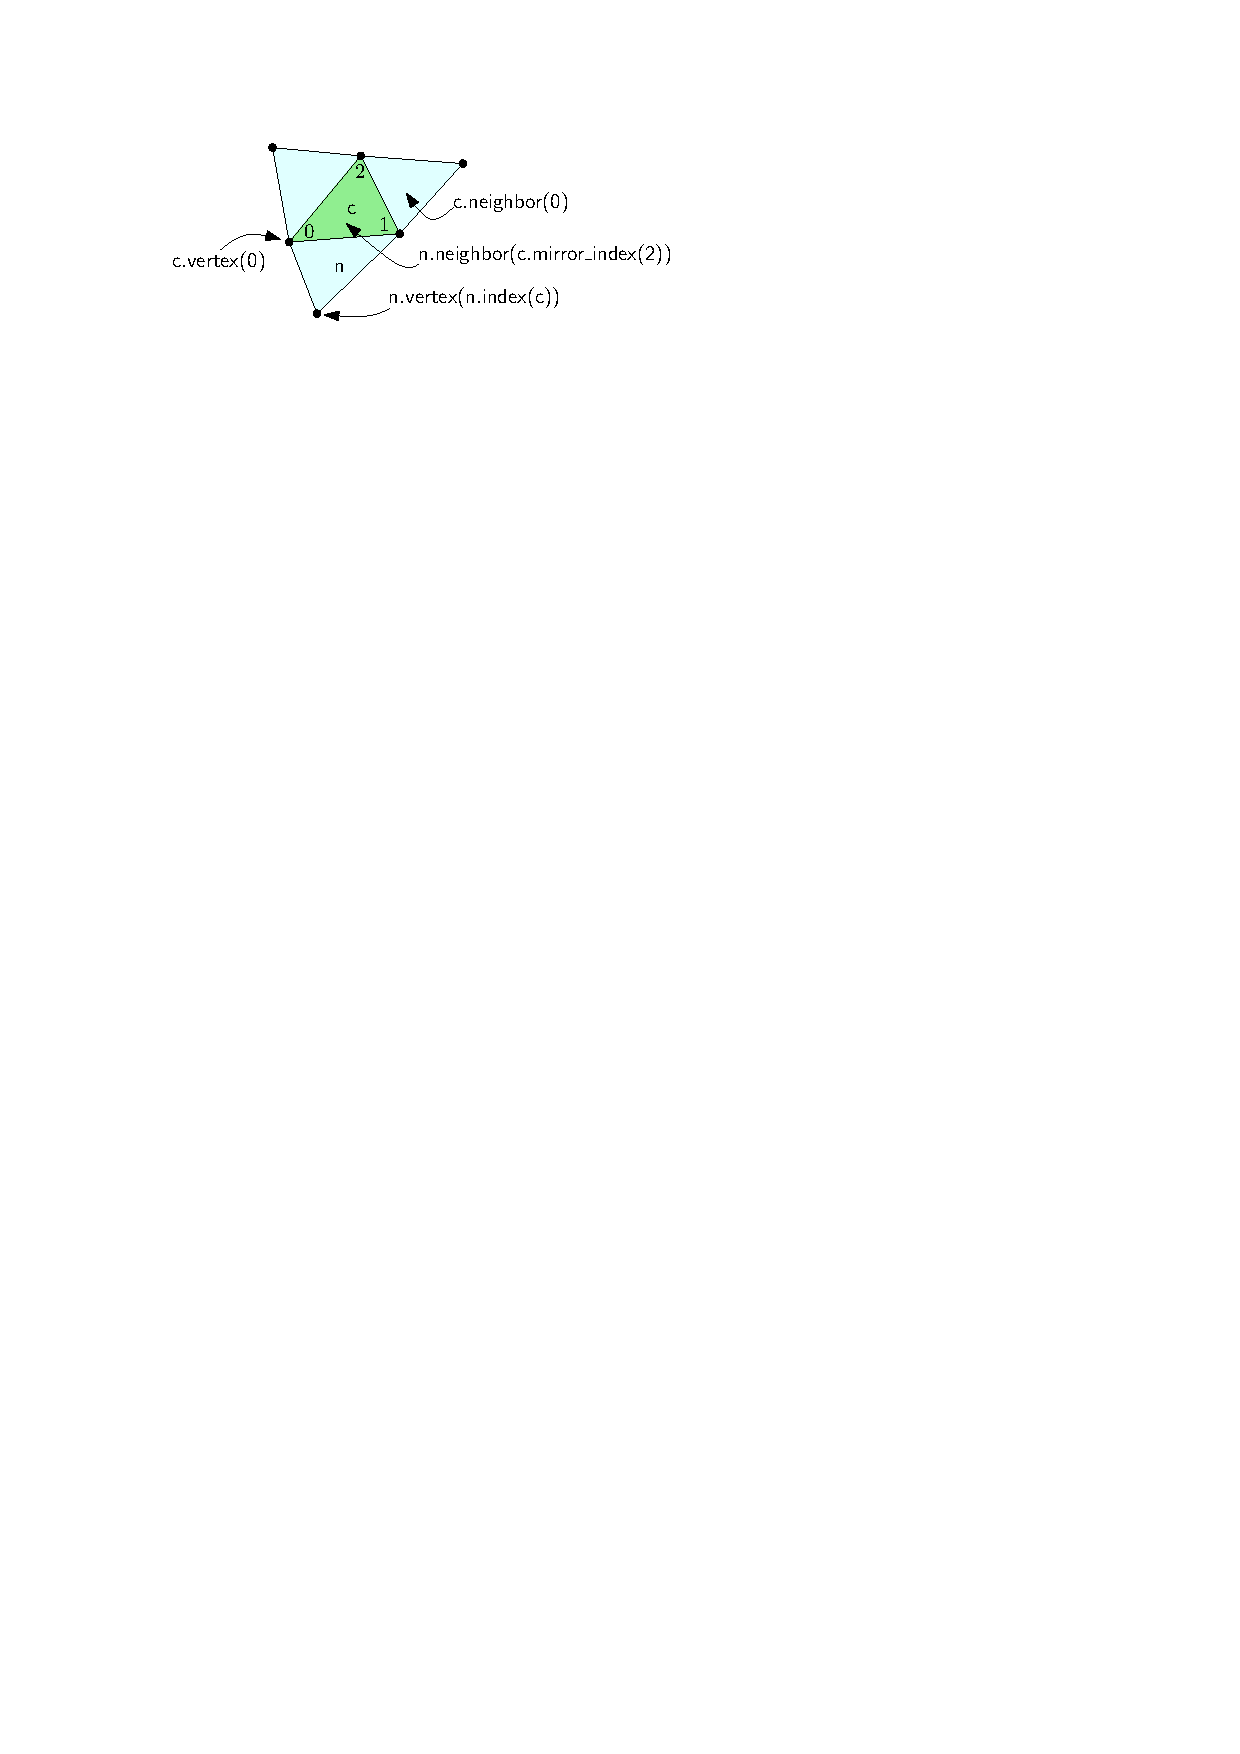
\includegraphics{Triangulation/fig/simplex-structure.pdf}
\end{center}
\end{ccTexOnly}
\begin{ccHtmlOnly}
<center>
<img border=0 src="./fig/simplex-structure.png" align="middle" alt="Index the vertices and neighbors of a simplex">
</center>
\end{ccHtmlOnly}
\caption{Indexing the vertices and neighbors of a simplex $s$.}
\label{triangulation:fig:simplex}
\end{figure} 

\paragraph{Instanciating the class template}

The \ccc{Triangulation_data_structure<Dimensionality, TDSVertex, TDSFullCell>}
class template is designed in such a way that its user can choose
\begin{itemize}
\item the ambient dimension of the triangulation data structure by specifying the \ccc{Dimensionality} template parameter,
\item the type used to represent vertices by specifying the \ccc{TDSVertex}
template parameter and
\item the type used to represent simplices by specifying the
\ccc{TDSFullCell} template parameter.
\end{itemize}

The last two parameters have default values and are thus not necessary, unless
the user needs custom types (see the reference manual page for this class
template). The first template parameter, \ccc{Dimensionality}, must be either
\begin{itemize}
\item \ccPureGlobalScope\ccc{Dimension_tag<D>} for some integer \ad. This
indicates that the pure complex can store simplices of dimension at most
\ad. The maximum dimension \ad\ is known by the compiler, which
triggers some optimizations. Or
\item \ccPureGlobalScope\ccc{Dynamic_dimension_tag}. In this case, the maximum
dimension of the simplices must be passed as an integer argument to an instance
constructor (see \ccc{TriangulationDataStructure}).
\end{itemize}

The \ccc{TDSVertex} and \ccc{TDSFullCell} parameters to the class template
must be models of the concepts \ccc{TriangulationDSVertex} and
\ccc{TriangulationDSFullCell} respectively. \cgal\ provides models for these
concepts: \ccc{Triangulation_ds_vertex<TDS>} and
\ccc{Triangulation_ds_simplex<TDS, TDSFullCellStoragePolicy>}, which, as one
can see, take the \tds\ as a template parameter in order to get access to
some nested types in \tds.

\textbf{This creates a circular dependency}, which we resolve in the same way
as in the \cgal\ \ccc{Triangulation_3} package (see
Chapters~\ref{chapter-TDS3}~and~\ref{chapter-Triangulation3}).
Thus, models of the concepts \ccc{TriangulationDSVertex} and
\ccc{TriangulationDSFullCell} must provide a nested template \ccc{Rebind_TDS}
which is documented in those two concept's reference manual pages.

\begin{ccAdvanced}
Thus, to the user in need of a custom vertex of simplex class, we recommend
the reading of the documentation of the \cgal\ \ccc{Triangulation_3} package.
\end{ccAdvanced}

% - - - - - - - - - - - - - - - - - - - - - - - - - - - - - - TDS EXAMPLES

\subsection{Examples\label{triangulation:tds:examples}}
 
\paragraph{Incremental Construction}
The following example shows how to construct a triangulation data structure by
inserting vertices. The reader will make the best use of this example by
reading it slowly, together with the reference manual documentation of the
methods that are called (see here: \ccc{TriangulationDataStructure}).

\ccIncludeExampleCode{Triangulation/triangulation_data_structure.cpp}


% - - - - - - - - - - - - - - - - - - - - - - - - - - - - - - TRIANGULATIONS

\section{Triangulations}

The class \ccc{CGAL::Triangulation<TrTraits, TDS>} embeds an abstract 
triangulation into euclidean space. More precisely, it
maintains a triangulation (a partition into pairwise interior-disjoint full
cells) of the convex hull of the points (the embedded vertices) of the
triangulation, as well as a triangulation of the complement of the convex hull
\textbf{in the affine subspace} spanned by the triangulation's points.

Methods are provided for the insertion of points in the triangulation, the
contraction of faces, the traversal of various elements of the triangulation
as well as the localization of a query point inside the triangulation.

Infinite cells outside the convex hull are each incident to
a finite facet on the convex hull of the triangulation and to a unique special
\textbf{vertex at infinity}. 
\note{In every infinite cell, the vertex at infinity
always has index $0$.}
\note{SH: the above note this should go in the documentation of the
\ccc{TriangulationDataStructure} concept, or that of the class?}

As long as no \emph{advanced} class method is called, it is guaranteed that
all finite cells have positive orientation. The infinite cells are
oriented so that the convex hull of the triangulation lies on the negative side of
the oriented hyperplane defined by the cell's finite facet.


% - - - - - - - - - - - - - - - - - - - - - - - - - Triangulation IMPLEMENTATION

\subsection{Implementation}

The class \ccc{CGAL::Triangulation<TrTraits, TDS>} stores a model \ccc{TDS}
of the concept \ccc{TriangulationDataStructure} which is instanciated with a
vertex type that stores a point, and a full cell type that allows the retrieval
of the point of its vertices.

The template parameter \ccc{TrTraits} must be a model of the concept
\ccc{TriangulationTraits} which provides the geometric \ccc{Point} type as well
as various geometric predicates used by the \ccc{Triangulation} class.

% - - - - - - - - - - - - - - - - - - - - - - - - - - - - Triangulation EXAMPLES

\subsection{Examples}

\paragraph{Incremental Construction}

The following example shows how to construct a triangulation in which we insert
random points. In \ccc{STEP 1}, we generate one hundred random points in
$\real^5$, which we then insert into a triangulation. In \ccc{STEP 2}, we 
%have a little fun and 
ask the triangulation to construct the set of edges
($1$-cells) incident to the vertex at infinity. It is easy to see that
these edges are in bijection with the vertices on the convex hull of the
points. This gives us a handy way to count the convex hull vertices. (Note that
in general, this set of vertices is a superset of the set of extremal vertices
of the convex hull.)

\ccIncludeExampleCode{Triangulation/triangulation.cpp}

\paragraph{Traversing the facets of the convex hull}

Remember that a triangulation triangulates the convex hull of its points. Each
facet of the convex hull is incident to one finite cell and one infinite
cell. In fact there is a bijection between the infinite cells and the
facets of the convex hull. So, in order to traverse the convex hull facets,
there are (at least) two possibilities:

The first is to iterate over the cells of the triangulation and check if they
are infinite or not:

\begin{ccExampleCode}
Triangulation t;

// ... insert points in the triangulation here.

typedef Triangulation::Full_cell_iterator Full_cell_iterator;
typedef Triangulation::Facet Facet;

for( Full_cell_iterator sit = t.full_cells_begin(); sit != t.full_cells_end(); ++sit )
{
    if( t.is_finite(sit) )
        continue;
    Facet ft(sit, 0); // |ft| is a facet of the convex hull
}
\end{ccExampleCode}
(\textbf{Remark}: the code example above will not compile unless you provide
the missing \ccc{typedef}s and variables declarations.)

A second possibility is to ask the triangulation to gather all the cells
incident to the infinite vertex: they form precisely the set of infinite
cells:

\begin{ccExampleCode}
Triangulation t;

// ... insert points in the triangulation here.

typedef Triangulation::Full_cell_handle Full_cell_handle;
typedef Triangulation::Facet Facet;
typedef std::vector<Full_cell_handle> Full_cells;

Full_cells infinite_full_cells;
std::back_insert_iterator<Full_cells> out(infinite_full_cells);

t.incident_full_cells(t.infinite_vertex(), out);

for( Full_cells::iterator sit = infinite_full_cells.begin(); sit != infinite_full_cells.end(); ++sit )
{
    Facet ft(*sit, 0); // |ft| is a facet of the convex hull
}
\end{ccExampleCode}
(\textbf{Remark}: the code example above will not compile unless you provide
the missing \ccc{typedef}s and variables declarations.)

One important difference between the two examples above is that the first uses
\emph{little} memory but traverses \emph{all} the cells, while the second
visits \emph{only} the infinite cells but stores handles to them into a
\emph{potentially big} array.

% - - - - - - - - - - - - - - - - - - - - - - - - - - - - - DELAUNAY TRIANGULATIONS

\section{Delaunay triangulations}%and regular triangulationes}

The class \ccc{CGAL::Delaunay_triangulation<DTTraits, TDS>} derives from
\ccc{CGAL::Triangulation<DTTraits, TDS>} and adds further constraints to a
triangulation, in that all its cells must have the so-called
\textbf{Delaunay} or \textbf{empty-ball} property: the interior of a ball
circumscribing any face of a Delaunay cell must be free from any vertex
of the triangulation.

The \textbf{circumscribing sphere} of a face \ccc{s} is the smallest sphere
touching all vertices of the face. A triangulation of the convex
hull of a finite point set has the Delaunay (or empty-ball) property if all
its cells have the Delaunay (or empty-ball) property:

Informally, a finite cell has the Delaunay (or empty-ball) property---with
respect to the triangulation---if no vertex of the triangulation lies in the
interior of its circumscribing sphere.

When a new point \ccc{p} is inserted into a Delaunay triangulation, the set of
finite cells whose circumscribing sphere contains \ccc{p} are said to
\textbf{be in conflict} with point \ccc{p}. The set of cells that are in
conflict with \ccc{p} form the \textbf{conflict zone}. That conflict zone is
augmented with the infinite cells whose finite facet does not lie
anymore on the convex hull of the triangulation (with \ccc{p} added). The cells
in the conflict zone are removed, leaving a hole that contains \ccc{p}. That
hole is then re-triangulated in a ``star shape'' centered at \ccc{p}.

Delaunay triangulation also supports vertex removal.

% - - - - - - - - - - - - - - - - - - - - - - - - - DELAUNAY IMPLEMENTATION

\subsection{Implementation}

The class \ccc{CGAL::Delaunay_triangulation<DTTraits, TDS>} derives from
\ccc{CGAL::Triangulation<DTTraits, TDS>}. It thus stores a model \ccc{TDS} of
the concept \ccc{TriangulationDataStructure} which is instanciated with a vertex
type that stores a geometric point, and a full cell type that allows the
retrieval of the point of its vertices.

The template parameter \ccc{DTTraits} must be a model of the concept
\ccc{DelaunayTriangulationTraits} which provides the geometric \ccc{Point} type as
well as various geometric predicates used by the \ccc{Delaunay_triangulation} class.
The concept \ccc{DelaunayTriangulationTraits} refines the concept
\ccc{TriangulationTraits} by requiring a few other geometric predicate necessary
for the computation of Delaunay triangulations.

% - - - - - - - - - - - - - - - - - - - - - - - - - - - - DELAUNAY EXAMPLES

\subsection{Examples}

\paragraph{Access to the conflict zone and created cells during point
insertion}

When using a cell type containing additional custom information, it may be
useful to get an efficient access to the cells that are going to be erased
upon the insertion of a new point in the Delaunay triangulation, and to the newly
created cells. The code example below shows how one can have efficient
access to both the conflict zone and the created cells, while still
retaining an efficient update of the Delaunay triangulation.

(\textbf{Remark}: the code below will not compile unless you provide the
missing \ccc{typedef}s and variables declarations.)

\begin{ccExampleCode}
Delaunay_triangulation t;
Vertex_handle v;
// Conflict zones in dimension 0 or 1 are pretty boring.
assert( 2 <= t.current_dimension() );

// We insert the points stored in the vector |points|.
for( pit = points.begin(); pit != points.end(); ++pit )
{
    Face             f = t.make_empty_face();
    Facet            ft;
    Full_cell_handle c;
    Locate_type      lt;

    c = t.locate(*pit, lt, f, ft, v);

    if(    lt == Delaunay_triangulation::ON_VERTEX
        || lt == Delaunay_triangulation::OUTSIDE_AFFINE_HULL )
    {
        // There is, a priori, no full_cell of interest here.
        v = t.insert(*pit, lt, f, ft, s);
    }
    else
    {
        typedef std::vector<Full_cell_handle> Full_cells;
        Full_cells zone, new_full_cells;
        std::back_insert_iterator<Full_cells> out(zone);
        Facet ftc = t.compute_conflict_zone(*pit, s, out);
        /*----------------------------------------------------\
        | Here, do something with the conflict zone cells     |
        | stored in |zone|.                                   |
        | DO NOT MODIFY the vector |zone|.                    |
        \----------------------------------------------------*/
        out = std::back_inserter(new_full_cells);
        v = t.insert_in_hole(p, zone.begin(), zone.end(), ftc, out);
        /*----------------------------------------------------\
        |  Here, do something with the newly created cells    |
        |  stored in |new_full_cells|.                        |
        \----------------------------------------------------*/
    }
}
\end{ccExampleCode}

\section{Complexity and performances}

\note{todo}

\section{Design and Implementation History}

This package is heavily inspired by the works of
 Monique Teillaud and Sylvain Pion (\ccc{Triangulation_3})
and Mariette Yvinec (\ccc{Triangulation_2}).
The first version was written by Samuel Hornus and then
pursued by Samuel Hornus and Olivier Devillers.
